\section{The Standard Model}
\label{SM}
\subsection{The Standard Model overview}
The underlying theory of modern High Energy Physics is the Standard Model (SM). This theory has been developed in the second half of the 20th century with contributions from many scientists and it is a very successful representation of the world on subatomic level.
SM classifies all known subatomic particles into specific categories and provides the description of the interactions between them. 

In SM there are two main types of fermions (1/2-spin particles) known as quarks and leptons. Each family has three generations with each consecutive generation being heavier than the previous. The lightest fermions (up \& down quarks + electron)
are stable and constitute ordinary matter. The interactions between fermions are mediated through the exchange of force carrier particles known as gauge bosons (see Tab.~\ref{tab:SM}). The final piece in SM is the Higgs boson and it gives mass to other fundamental particles. All bosons possess and integer spin \citep{martin2006nuclear}. 
\begin{table}[]
\centering
\label{my-label}
\begin{tabular}{cccc | ll}
\textbf{Fermion}                  & \multicolumn{3}{c}{\textbf{Generations}} & \multicolumn{2}{c}{\textbf{Bosons}} \\ \hline
\multirow{2}{*}{\textbf{Leptons}} & $e$        & $\mu$        & $\tau$       & $Z$            & Higgs           \\
                                  & $\nu_{e}$  & $\nu_{\mu}$  & $\nu_{\tau}$ & $W^{\pm}$            &                 \\ 
\multirow{2}{*}{\textbf{Quarks}}  & $u$        & $c$          & $t$          & photon            &                 \\
                                  & $d$        & $s$          & $b$          & gluon             &          \\ \hline      
\end{tabular}
\caption{The Standard Model particles}
\label{tab:SM}
\end{table}

The mathematical representation of SM is built within the broader frame of Group Theory.  SM has the symmetry group U(1)$_{\text{Y}}\times$SU(2)$_{\text{L}}\times$SU(3). The SU(3) symmetry group generates strong interactions, that describe processes involving quarks and gluons. The U(1)$_{\text{Y}}\times$SU(2)$_{\text{L}}$ generates electroweak interactions. At the energies below 100 GeV, however, the single electroweak interaction is broken into the weak and electromagnetic varieties with the symmetry group U(1)$_{\text{em}}$. 
The unification of these two types was the result of efforts by Glashow, Weinberg and Salam \citep{Glashow:1961tr,weinberg1967model,salam1968elementary}. 
The weak interaction processes involve fermions and are mediated by electrically charged W\textsuperscript{$\pm$} for charged processes and chargeless Z gauge bosons for neutral ones. Electromagnetic force is mediated by photons and only involves electrically charged particles. 

Above the unification energy of 100 GeV,and thus before the spontaneous electroweak symmetry breaking  through Higgs mechanism \citep{englert1964broken, higgs1964broken}, the gauge bosons are different. There are three W bosons, denoted W\textsuperscript{1}, W\textsuperscript{2}, W\textsuperscript{3} corresponding to SU(2)$_{\text{L}}$ part of the group and one B boson corresponding to U(1)$_{\text{Y}}$. 
All the electroweak bosons are massless, and acquire mass by coupling to the Higgs field in the process of symmetry breaking.  

\subsection{The Standard Model limitations}

The SM predictions have been successfully tested in particle accelerator experiments, and the final confirmation came with the discovery of the Higgs boson in 2012 - a true scientific breakthrough \citep{Aad:2012tfa}\citep{chatrchyan2012observation}. This was the last missing piece of experimental evidence needed for the full validation of SM. The experiments that led to this discovery were conducted at CERN’s Large Hadron Collider (LHC) in run-1 proton-proton collisions at centre-of-mass energy $\sqrt{s}=$7 and the later upgrade to 8 TeV.  
Despite the fact that SM has proven to be an extremely precise and successful theory there are some caveats for which it does not provide  adequate solutions. 

One of the inconsistencies within SM is the so-called Hierarchy problem \citep{PhysRevD.14.1667}. One of the ways it reveals itself is through the large discrepancy between the Planck mass and the mass of the Higgs particle. The former is about $10^{17}$ times bigger than the latter and current representation of particle physics cannot explain such a big difference. Quantum effects start manifesting themselves at the Plank mass threshold and such a vast difference between these two values is yet unaccounted for. 

Another prominent problem is that SM does not explain dark matter. While ordinary matter only constitutes about 5\% in the total mass-energy content of the universe, it is dark matter and dark energy that account for the rest \citep{ade2014planck}. 
%However,
SM does not provide a candidate particle for dark matter and thus is only able to describe ordinary matter and energy. 

One of the main challenges of modern physics is the unification of forces. This is part of the ongoing attempts to reach the ultimate goal - a "theory of everything". Such a theory would have to account for all physical aspects of the universe and include the most fundamental structures and interactions. The first step was made with the unification of electromagnetic and weak forces.  
The next step is to achieve the unification of electromagnetic, weak, and strong interaction forces – this step is called the Grand Unification. The ultimate step is to combine all four fundamental forces together, which means adding gravity, in what is called Super Unification (see Fig.~\ref{fig:unification}). Thus far quantum field theory and general relativity are able to describe phenomena on their respective scale of action with remarkable precision, but are fundamentally incompatible.  
\begin{figure}[ht]
		\centering
			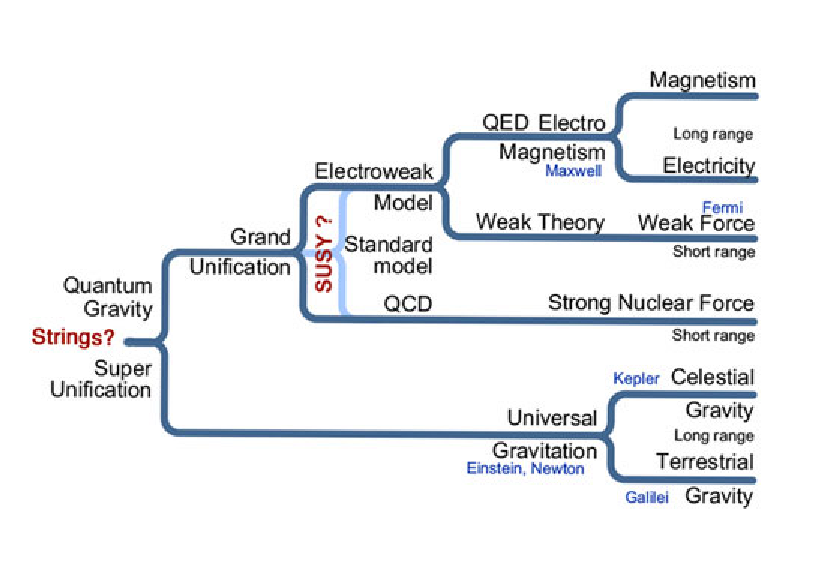
\includegraphics[scale=0.8]{Chap2/Unification}
\caption{\label{fig:unification} Various stages in the unification of forces  \citep{unification}}.
\end{figure}

Within the confines of the Standard Model even the Grand Unification is not possible, and this prompts the search for new theories that account for this and other shortcomings of SM. Collectively they are called Beyond-Standard-Model (BSM) theories. Among these there are theories that include extra-dimensions, composite Higgs boson models, etc. Theoretical and experimental search for BSM physics is the current frontier in high energy physics and one of the most important questions in science overall. 


\section{Supersymmetry}
One of the strongest candidate framework theories that can offer solutions to SM deficiencies is Supersymmetry (SUSY) \citep{Lykken:1996xt}. SUSY is a spacetime symmetry that equates fermionic and bosonic degrees of freedom. Among several theories that are based on SUSY principles, the Minimal Supersymmetric Standard Model (MSSM) offers the simplest extention of SM. MSSM postulates that each SM particle has a supersymmetric partner which is  different only in spin by one-half unit (see Table~\ref{tab:MSSMparticles}), while all other quantum numbers stay the same. 
\vspace{0.5cm}
\begin{table}
\captionsetup{width=0.8\textwidth}
\def\arraystretch{1.5}
\centering
\begin{tabular}{|l|c| l|}
\hline 
name & spin & particles \\ 
\hline 
squarks & 0 & $\tilde{d}_{L},\tilde{u}_{L},\tilde{s}_{L},\tilde{c}_{L}, \tilde{b}_{1}, \tilde{t}_{1}, \tilde{d}_R,\tilde{u}_{R},\tilde{s}_{R},\tilde{c}_{R},\tilde{b}_{2}, \tilde{t}_{2} $\\ 
sleptons & 0 & $\tilde{e}_L, \tilde{\nu}_{eL}, \tilde{\mu}_L, \tilde{\nu}_{\mu L}, \tilde{\tau}_1, \tilde{\nu}_{\tau L}, \tilde{e}_R,\tilde{\mu}_R, \tilde{\tau}_2 $\\ 
charginos & $1/2$ & $\tilde{\chi}_1^{\pm} ,\, \tilde{\chi}_2^{\pm}  $ \\ 
neutralinos & $1/2$ & $\tilde{\chi}_1^{0},\, \tilde{\chi}_2^{0},\,\tilde{\chi}_3^{0},\, \tilde{\chi}_4^{0} $\\ 
gluino & $1/2$ & $\tilde{g}$ \\  
Higgs & 0 & $h^{0},\, H^{0},\, A^{0},\, H^{\pm}$ \\ 
\hline 
\end{tabular} 
\caption{\label{tab:MSSMparticles} SUSY particles in MSSM where subscript $R$ denotes right-handed particles and $L$ - left-handed ones. $H^0$ Higgs boson also exists in SM. }
\end{table}
The superpartners of quarks, leptons, and neutrinos are called squarks, sleptons and sneutrinos. For gauge bosons the superpartners are  gluinos, photino, winos and binos, collectively named gauginos. The latter two are superpartners of the  B and three W bosons of the elecroweak interaction before electroweak symmetry breaking. It follows naturally since SUSY is invoked before the electroweak symmetry breaking. The Higgs sector in SUSY has five superpartners  - two charged $(H^{\pm})$ sparticles and three neutral ones $(h^0, H^0, A^0)$. They are known collectively as Higgsinos. Mixing between winos, binos and Higgsinos results in charginos and neutralinos. Their mass eigenstates are referred to as $\tilde{\chi}^{\pm}_{i}$ ($i$ = 1,2) and $\tilde{\chi}^{0}_{i}$ ($i$ = 1,2,3,4) in order fo increasing mass. 

MSSM belongs to a class of theories that all share the same requirement - a quantity known as R-parity has to be conserved in interactions. The mathematical description of R-parity is beyond the scope of this paper. However, one important consequence of R-parity conservation is that if supersymmetric particles were to be produced in collisions, they will be created in pairs. Then they decay through various possible scenarios with the lightest supersymmetric particle (LSP) emerging in the final state and escaping undetected. The LSP is stable and provides a possible candidate for the dark matter particle.

The MSSM imposes 105 free parameters and it is one of its major issues, since any analysis will be addled with enormous complexity. There are various simplified models that reduce the number of free parameters to manageable values through various theoretically and experimentally motivated constraints. One them is the phenomenological Minimal Supersymmetric Standard Model (pMSSM) that contains only 19 free parameters and it will be used in this thesis' analysis. 





\section{The ATLAS detector}
\label{sec:atlas}
The ATLAS experiment is a multi-purpose particle detector with cylindrical geometry and has a nominal forward-backward symmetry \citep{aad2008atlas}. The dimensions of the detector are 25 m in height and 44 m in length and the overall weight of the detector is approximately 7000 tonnes.
It can detect particles with almost 4$\pi$ coverage in solid angle around the collision point, which covers almost all of the spherical area around the center. 

Proton bunches are accelerated in the underground ring that is 27 km in diameter and are directed to collide inside the detectors. The collisions happen at 40 MHz bunch crossing rate, with an average 25 interactions per bunch crossing. The LHC is designed to operate at $\sqrt{s}$=14 TeV and instantaneous luminosity $\mathcal{L} = 10^{34}$ cm\textsuperscript{-2} s\textsuperscript{-1} in proton-proton collision mode. Instantaneous luminosity is defined as follows
\begin{equation}
\mathcal{L} = \frac{1}{\sigma}\frac{dN}{dt}
\end{equation}  
Where $\sigma$ is the interaction cross-section, and $N$ is the number of detected events during time $t$. Integrated luminosity $\int \mathcal{L}\, dt$ is a quantity that expresses the amount of total data gathered during the time $t$ of running the LHC. The analysis presented in this paper uses the dataset recorded at 3.2 fb\textsuperscript{-1} of integrated luminosity throughout run-II during 2015.  
\begin{figure}[!t]
	\centering
    \captionsetup{width=\textwidth}
	\includegraphics[width=\textwidth]{Chap2/ATLAS_SE_WithDimensions_Corrected.png}
\caption{\label{fig:detector}  Cut-away view of the ATLAS detector (people are included for scale comparison) \citep{aad2008atlas}. }
\end{figure}

The Cartesian coordinate system used at ATLAS has its origin at the nominal point of interaction with $z$ axis extending along the particle beam longitudinally, positive $x$ axis pointing towards the center of the ring, and positive $y$ axis pointing upwards. 
The geometry of the detector makes the use of cylindrical coordinate system especially convenient. In it, $z$ axis stays the same, the polar angle $\theta$ is the angle from $z$-axis, and the azimuthal angle $\phi$ encircles $z$ axis in the transverse plane. However, instead of $\theta$ it is more convenient to use pseudorapidity $\eta$, due to the fact that differences in pseudorapidity are close to invariant under boosts along the $z$ axis (fully invariant for real rapidity). $\eta$ is defined as follows
\begin{equation}
\eta = -\ln\biggl(\tan\frac{\theta}{2}\biggr)
\end{equation}

Within $x$-$y$ plane the transverse energy $E_{T}$ and transverse momenta $p_{T}$ are defined.

\subsection{ The ATLAS sub-detectors and trigger systems}

The ATLAS detector consists of subdetector layers that are particularly sensitive to a designated type of particles produced in proton-proton collisions (see Fig.~\ref{fig:event}). The Inner Detector is closest to the collision point and covers $|\eta|<2.5$ in pseudorapidity. It has high granularity as it is exposed to the highest density of particle interaction. It was designed to provide a transverse momentum resolution and a transverse impact parameter resolution \citep{aad2010atlas}.The detector itself consists of three separate subsystems. The main components of the Inner Detector are: silicon pixel detector, semiconductor tracker, and transition radiation tracker. The three layers are all immersed in a 2 T magnetic field, created by the thin superconducting solenoidal magnet. This field is parallel to the beam axis and bends trajectories of charged particles allowing their charge and momentum identification based on the characteristic bending of their trajectories. 
\begin{figure}[!h]
	\centering
    \captionsetup{width=\textwidth}
	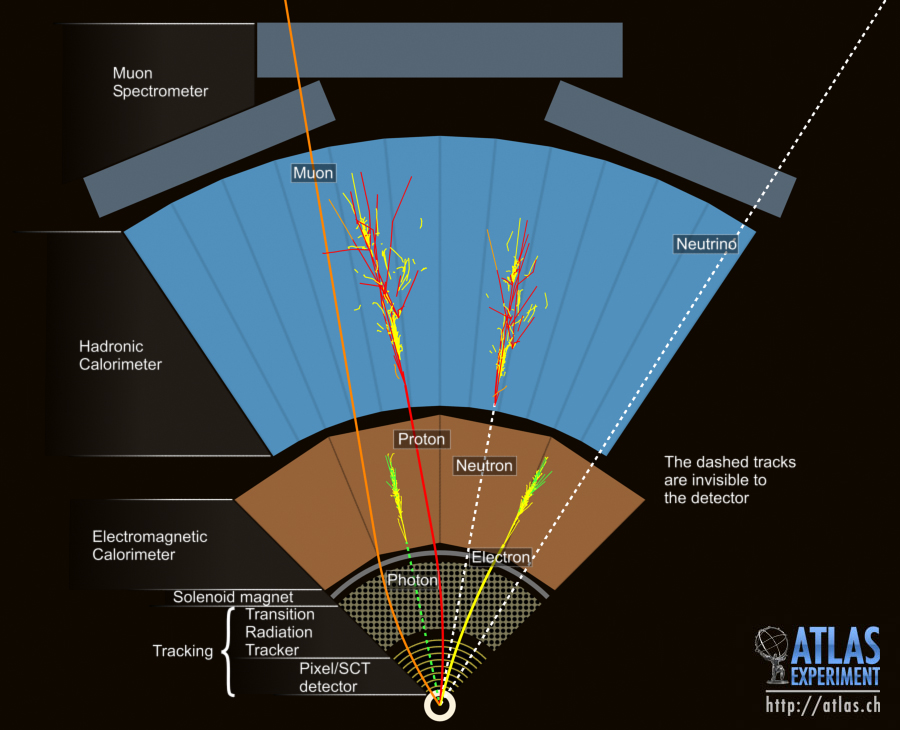
\includegraphics[width=0.9\textwidth]{Chap2/0803022_01.jpg}
\caption{\label{fig:event} Event in the transverse plane, a computer generated image of the ATLAS detector \cite{event}. }
\end{figure}

The next two layers are the two calorimeters that measure energies of specific type of particles. The particles travel through the detectors and lose their energy through interaction with its layers leaving energy deposits as they move through the material. 
The first one is the high-granularity Electromagnetic Calorimeter (EmCal) and it measures energies of electrons and photons. Colored particles (gluons and quarks) travel further into Hadronic calorimeter (HCal) where they continue their decays and also deposit their available energy. 
Both calorimeters are  designed to provide good quality measurements of momentum and energy and cover the region $|\eta|<4.9$.

The final detecting layer is the Muon spectrometer, which tracks and measures charged particles, specifically muons. It is immersed into a large toroidal magnet, that provides a magnetic field throughout the spectrometer and bends the trajectories of charged muons, which makes it possible to detect their charge and momentum. Any particles that are not covered by the described sub-detectors will escape undetected. These include neutrinos and, possibly, the LSP. 

Triggers are used to select events by identifying signatures of various particles as well as using global event signatures, such as missing transverse energy \citep{aad2012performance}. A three-level trigger system is used at ATLAS to select events that are of interest to further offline analysis. 
The  first  level is hardware-based and uses information from the calorimeters and muon spectrometer, the second and third levels are software-based and use information from all sub-detectors. Because the data at LHC is produced in staggering amounts employing efficient trigger systems is crucial to be able to extract information that is relevant for further analysis. At $\sqrt{s}$=13 TeV the spacing between bunches crossing is 25 ns and the collision rate is 40 MHz. This rate has to be reduced to O(500 Hz) to keep data in permanent memory devices \citep{barr2015particle}.

Ideally, a trigger should be able to retain maximum number of events that are interesting for physics analysis and reject as many background events as possible. In this regard the concept of trigger efficiency is very important, and this efficiency varies depending on the particular process that is being investigated. The overall goal is to reduce data from the raw amount to the size at which data can be stored permanently and at the same time keep as many relevant events as possible. 
